\documentclass[12pt]{article}
\usepackage{array,tabularx}
\usepackage{graphicx}
\usepackage{float}
\usepackage{amsmath}
\setlength{\parindent}{0pt}

\newenvironment{conditions}
  {\par\vspace{\abovedisplayskip}\noindent
   \tabularx{\columnwidth}{>{$}l<{$}@{}>{${}}c<{{}$}@{} >{\raggedright\arraybackslash}X}}
  {\endtabularx\par\vspace{\belowdisplayskip}}

\title{Volumes of Arbitrary Shapes}
\author{Ben Hammond}
\date{\today}

\begin{document}
	\maketitle
	\newpage

	\section*{Introduction}
	In class we went over how to find the volumes of arbitrary, but simple shapes. These were only ever defined in one axis, or by a simple equation to determine a variable cross-section. This is a test area for finding the volumes of shapes defined in three dimensions by arbitrary equations.

	\section*{Tests}
	
	\paragraph{1a.}
	What is the functional form of the Gravitational Potential energy (U) for the Sun? (Hint: Integrate (anti-derivative) the Gravitational force with respect to r)

	\paragraph{Response:}
		The force of gravity was first found, such that
		\begin{equation}
			F = \frac{GM_cM_s}{r^2}
		\end{equation}
		where
		\begin{conditions}
			F   & = &  gravitational force \\
			G   & = &  $6.67 \times 10^{-11} \frac{\text{N } \cdot \mbox{ m}^2}{\text{kg}^2}$ \\
			M_c & = &  mass of the comet \\
			M_s & = &  mass of the sun \\
			r   & = &  distance from the comet to the sun
		\end{conditions}
		This equation was then simplified to
		\begin{equation}
			F = GM_cM_sr^{-2}
		\end{equation}
		By integrating the gravitational force with respect to r, the gravitational potential energy was found
		\begin{equation}
			\int{Fdr}
		\end{equation}
		\begin{equation}
			W = -GM_Cm_sr^{-1}
		\end{equation}
		\begin{equation}
		\label{grav_potential}
			U = \frac{-GM_cM_s}{r}
		\end{equation}


	\paragraph{1b.}
	Create a relatively accurate sketch of the comet's orbit. Identify the perihelion, aphelion, elliptical	foci, Oort cloud, Sun, and Earth.

	\paragraph{Response:}
		
		Using these values, a rough sketch was drawn
		\begin{figure}[H]
			\centerline{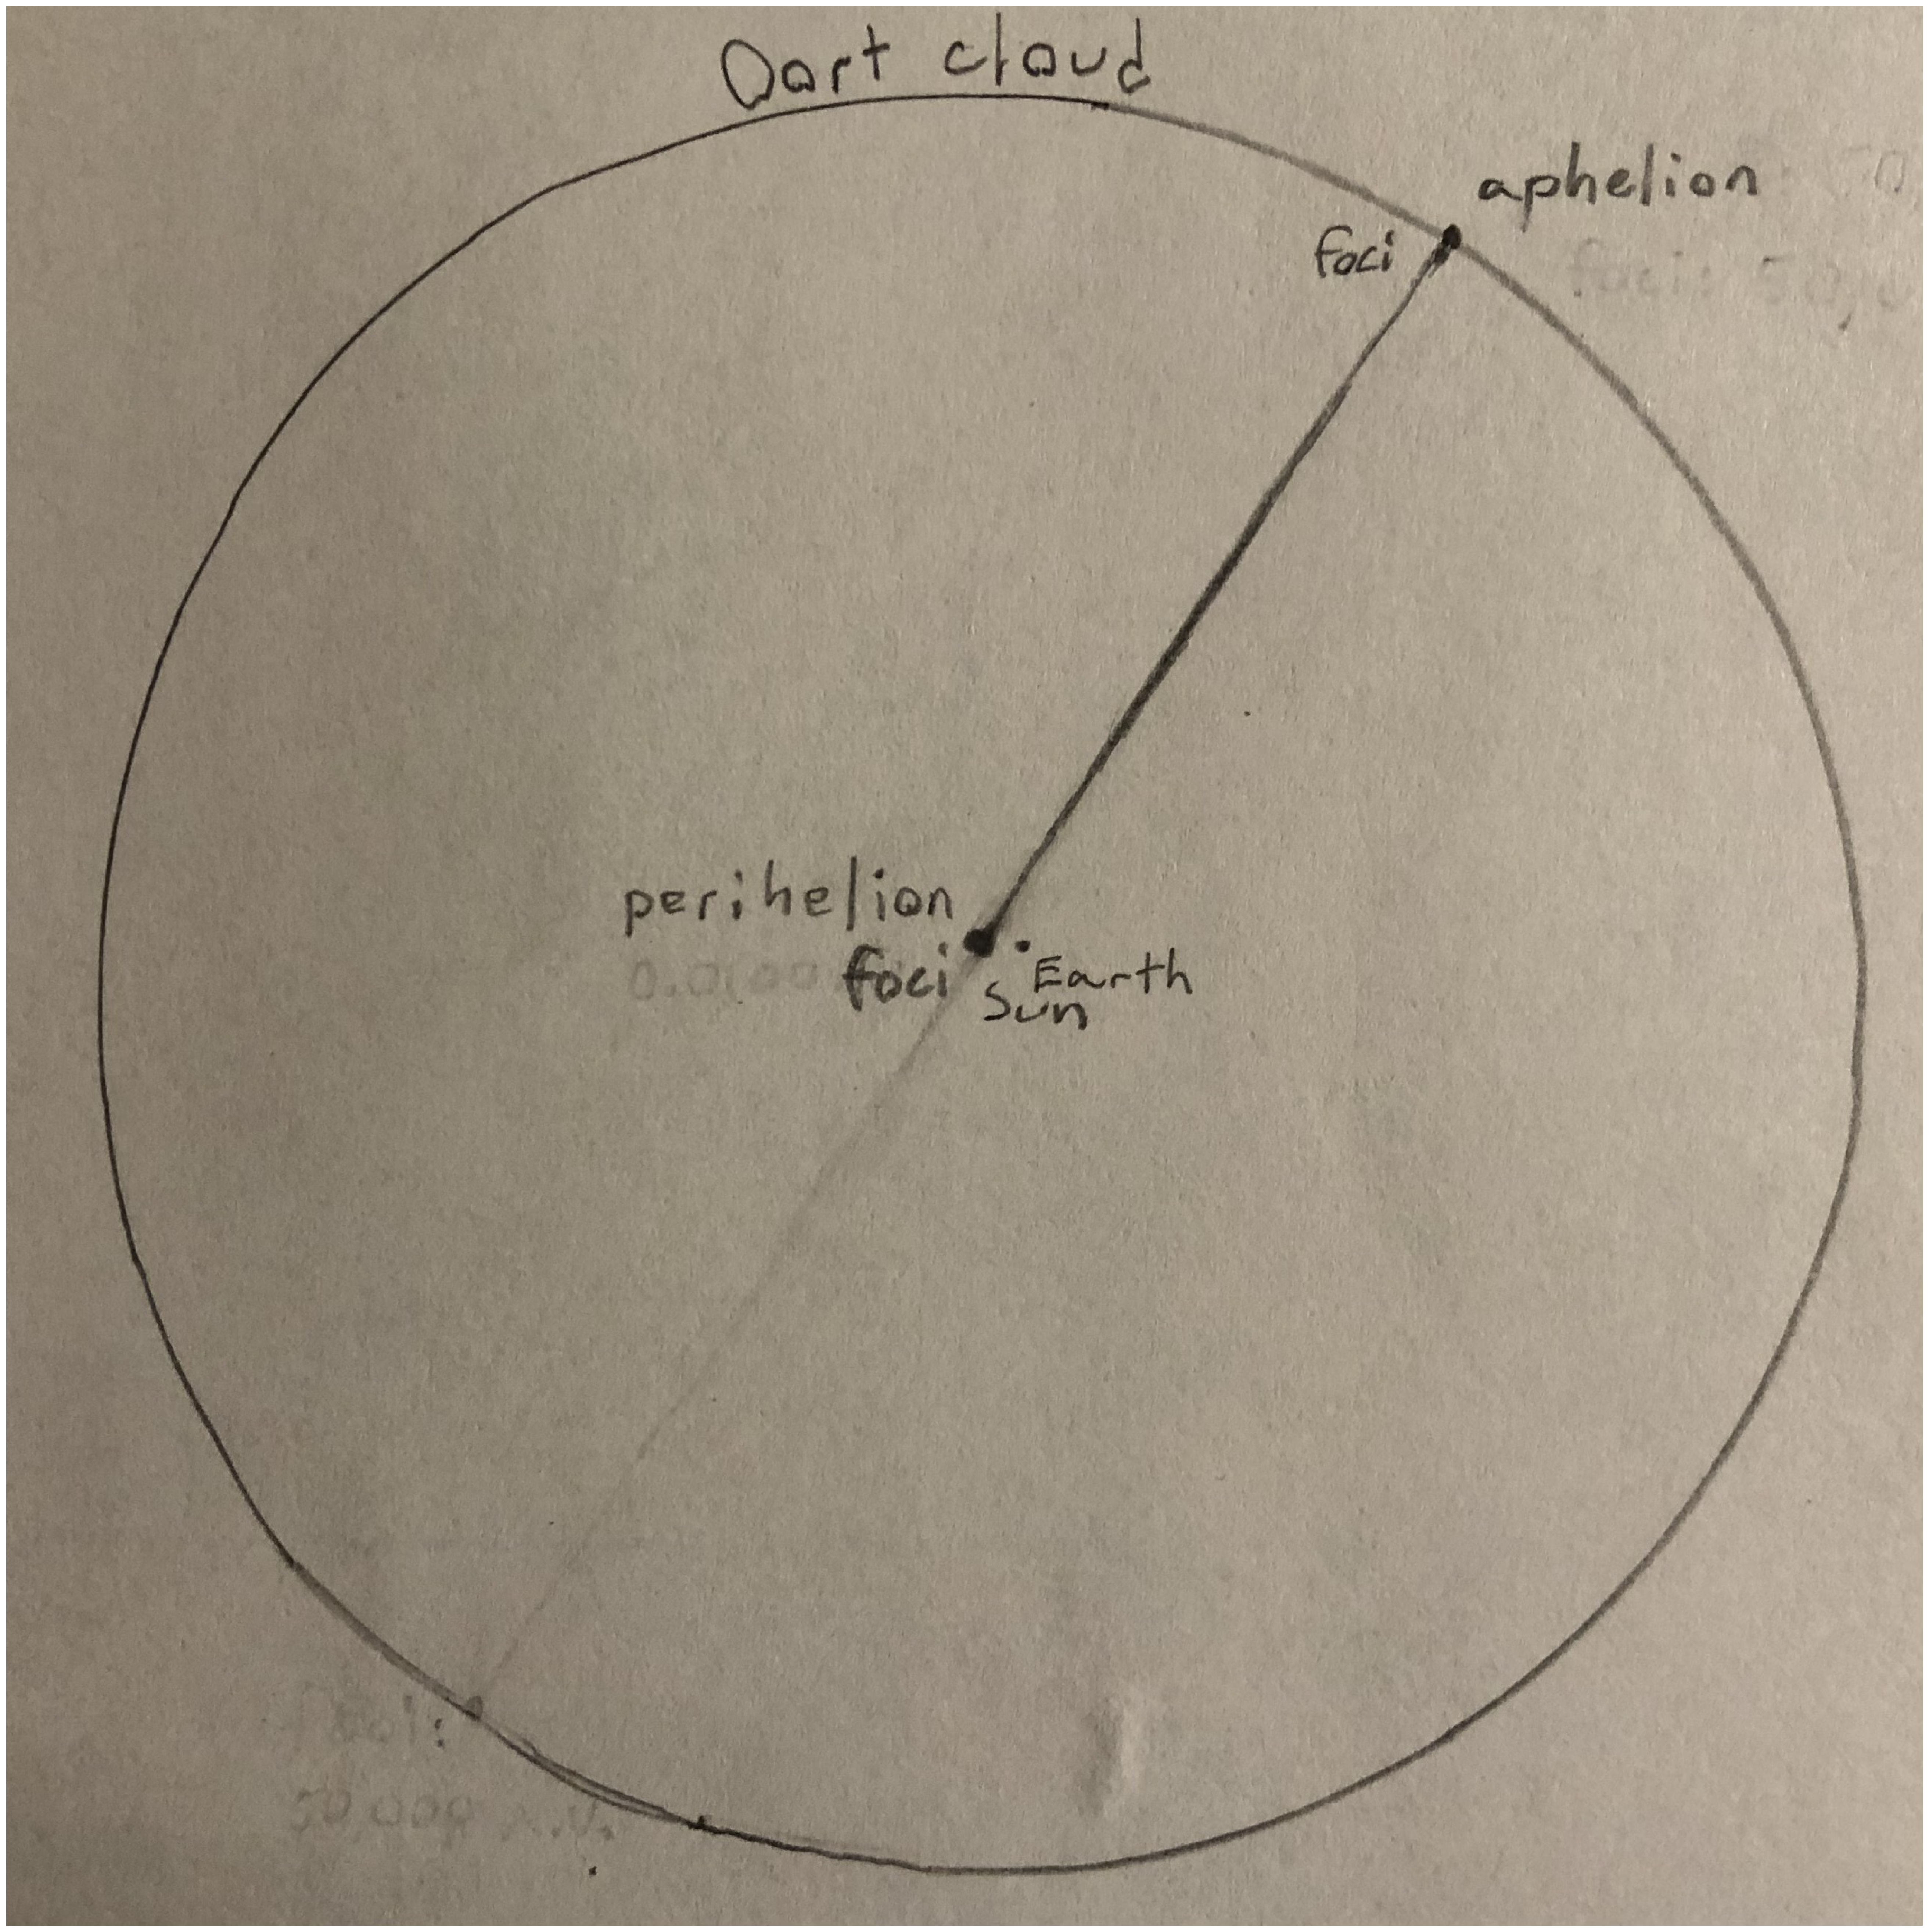
\includegraphics[width=0.5\textwidth]{orbital_overview.eps}}
			\caption{An orbital overview.}
		\end{figure}

	\paragraph{2.}
	Determine the velocity of the comet at its perihelion.

	\paragraph{Response:}
		By using the definition of kinetic energy as
		\begin{equation}
			KE = \frac{1}{2}mv^2 = PE_1 - PE_2
		\end{equation}
		where
		\begin{conditions}
			KE  & = &  kinetic energy \\
			m   & = &  mass (kg) \\
			v   & = &  velocity (m/s) \\
			PE  & = &  potential energy
		\end{conditions}
		and substituting $PE_1$ and $PE_2$ with the gravitational potential energy equation found in equation \ref{grav_potential}, the velocity can be isolated and solved for:
		\begin{equation}
			\frac{1}{2}M_cv^2 = \frac{-GM_cM_s}{r_p} - \frac{-GM_cM_s}{r_a}
		\end{equation}
		where
		\begin{conditions}
			M_s  & = &  mass of the sun ($1.99 \times 10^{30}$ kg) \\
			r_p  & = &  distance from the comet to the sun at perihelion \\
			r_a  & = &  distance from the comet to the sun at aphelion
		\end{conditions}
		\begin{equation}
			\frac{1}{2}v^2 = \frac{-GM_s}{r_p} - \frac{-GM_s}{r_a}
		\end{equation}
		\begin{equation}
			v = \sqrt{2 \left(\left(\frac{-GM_s}{r_p}\right) - \left(\frac{-GM_s}{r_a}\right)\right)}
		\end{equation}
		\begin{equation*}
			\resizebox{0.9\textwidth}{!}
				{%
					$ v = \sqrt{2\\
					\left(\\
					\left(\\
					\frac{-6.67 \times 10^{-11}\frac{\text{N } \cdot \text{ m}^2}{\text{kg}^2} \cdot 1.99 \times 10^{30} \text{ kg}}{(0.0100 \text{ A.U.})\left(1.50 \times 10^8 \frac{\text{km}}{\text{A.U.}}\right)\left(1000 \frac{\text{m}}{\text{km}}\right)}\\
					\right) -\\
					\left(\\
					\frac{-6.67 \times 10^{-11}\frac{\text{N } \cdot \text{ m}^2}{\text{kg}^2} \cdot 1.99 \times 10^{30} \text{ kg}}{(50000 \text{ A.U.})\left(1.50 \times 10^8 \frac{\text{km}}{\text{A.U.}}\right)\left(1000 \frac{\text{m}}{\text{km}}\right)}\\ 
					\right)\\
					\right)}$%
				}
		\end{equation*}
		$$ v = 348000 \text{m/s} $$


	\paragraph{3.}
	Using Kepler's second law, determine the velocity of the comet at aphelion.

	\paragraph{Response:}
		By using an expression of Kepler's second law:
		\begin{equation}
			v_a = v_p\left(\frac{h_p}{h_a}\right)
		\end{equation}
		where
		\begin{conditions}
			v_a  & = &  velocity of the comet at perihelion \\
			v_p  & = &  velocity of the comet at aphelion \\
			h_p  & = &  distance from the comet to the sun at perihelion \\
			h_a  & = &  distance from the comet to the sun at aphelion
		\end{conditions}
		and filling in known values as well as the perihelion velocity found from equation 5, the velocity of the comet at aphelion can be found
		$$ v_a = 348000\text{ m/s }\left(\frac{0.0100\text{ A.U.}}{50000\text{ A.U.}}\right) $$
		$$ v_a = 0.0696\text{ m/s} $$
		
	\paragraph{4.}
	Write an equation for the comet's elliptical orbit.
	
	\paragraph{Response:}
		With the equation for an ellipse as
		\begin{equation}
			\frac{x^2}{a^2} + \frac{y^2}{b^2} = 1
		\end{equation}
		where
		\begin{conditions}
			x  & = &  distance from the comet to the center of the ellipse in the horizontal axis \\
			y  & = &  distance from the comet to the center of the ellipse in the vertical axis \\
			a  & = &  distance from the center of the ellipse to either perihelion or aphelion \\
			b  & = &  distance from the horizontally widest point of the ellipse to its center
		\end{conditions}
		Though neither $a$ nor $b$ are known, $a$ is quickly solved for as follows
		\begin{equation}
			a = \frac{1}{2}(h_a + h_p)
		\end{equation}
		$$ a = \frac{1}{2}(50000.\text{ A.U.} + 0.0100\text{ A.U.}) $$
		$$ a = 25000.005\text{ A.U.} $$
		Though $b$ still cannot be found, $c$, the distance from the foci to the center of the ellipse, is solved for through
		\begin{equation}
			c = a - h_p
		\end{equation}
		$$ c = 25000.005\text{ A.U.} - 0.0100\text{ A.U.} $$
		$$ c = 24999.995\text{ A.U.} $$
		With $a$ and $c$ now found, $b$ is isolated from the equation
		\begin{equation}
			c^2 = a^2 - b^2
		\end{equation}
		\begin{equation}
			b = \sqrt{a^2 - c^2}
		\end{equation}
		and is solved for by inputting the known values of $a$ and $c$
		$$ b = \sqrt{(25000.005\text{ A.U.})^2 - (24999.995\text{ A.U.})^2} $$
		$$ b = 22.4\text{ A.U.} $$
		Thus, the equation for the ellipse of the comet's orbit is
		\begin{equation}
			\frac{x^2}{(2.50 \times 10^4 \text{ A.U.})^2} + \frac{y^2}{(22.4 \text{ A.U.})^2} = 1
		\end{equation}
		
	\paragraph{5.}
	What is the minimal velocity a comet must have at the Oort cloud to overcome the gravitational pull or the sun and escape the solar system?

	\paragraph{Response:}
		With the equation for escape velocity as
		\begin{equation}
			v = \sqrt{\frac{2GM_s}{r}}
		\end{equation}
		the escape velocity of the comet at aphelion is found:
		$$ v = \sqrt{\frac{2\left(-6.67 \times 10^{-11}\frac{\text{N } \cdot \text{ m}^2}{\text{kg}^2}\right) \cdot \left(1.99 \times 10^{30} \text{ kg}\right)}{(50000 \text{ A.U.})\left(1.50 \times 10^8 \frac{\text{km}}{\text{A.U.}}\right)\left(1000 \frac{\text{m}}{\text{km}}\right)}} $$
		$$ v = 188\text{ m/s} $$

	\paragraph{6.}
	Is the direction of the velocity in question 5 important? Explain.
	
	\paragraph{Response:}
		The direction of the velocity in question 5 is important. To escape the Sun's orbit the velocity must be tangent to the orbit at aphelion, as other directions may change the orbit but will not result in an orbital escape.
	
	\paragraph{7.}
	Use Kepler's third law to estimate the orbital period of the comet.

	\paragraph{Response:}
		Given a general form of Kepler's third law
		\begin{equation}
			\frac{T_c^2}{R_c^3} = \frac{T_e^2}{R_e^3}
		\end{equation}
		\begin{equation}
			T_c = \sqrt{R_c^3 \times \frac{T_e^2}{R_e^3}}
		\end{equation}
		where
		\begin{conditions}
			T_c  & = &  period of the comet's orbit (seconds) \\
			R_c  & = &  average radius of the comet's orbit (meters) \\
			T_e  & = &  period of the earth's orbit ($3.154\times10^7$ seconds) \\
			R_e  & = &  average radius of the earth's orbit ($1.496\times10^{11}$ meters)
		\end{conditions}
		and a calculated average orbit size of the comet
		\begin{equation}
			R_c = \frac{h_a + h_p}{2}
		\end{equation}
		$$ R_c = \frac{50000\text{ A.U.} + 0.0100\text{ A.U.}}{2} $$
		$$ R_c = 25000.005\text{ A.U.} $$
		the period can be found such that
		$$ T_c = \sqrt{\left(25000.005\text{ A.U.} * 1.496\times10^{11} \frac{\text{m}}{\text{A.U.}}\right)^3 \times \frac{(3.154\times10^7\text{ s})^2}{(1.496\times10^{11}\text{ m})^3}} $$
		$$ T_c = 1.24673 \times 10^{14}\text{ s} $$
		$$ T_c(\text{years}) = (1.24673 \times 10^{14}\text{ s}) * (3.17098 \times 10^{-8} \frac{\text{yr}}{\text{s}}) $$
		$$ T_c(\text{years}) = 3.95 \times 10^6 \text{ yr} $$
	
	\paragraph{8.}
	If the Sun had the same radius as the earth ($6.38 \times 10^6$ m), what velocity would the comet have if it passed within 100. km of the surface?

	\paragraph{Response:}
		The new perihelion was found by summing the radius of the earth and the comet's distance above the surface:
		$$ h_p = 6.38 \times 10^6\text{ m} + 1.00 \times 10^5\text{m} $$
		$$ h_p = 6.48 \times 10^6\text{ m} $$
		With the new perihelion, equation \ref{grav_potential} was used to find the comet's velocity at perihelion
		\begin{equation*}
			\resizebox{0.9\textwidth}{!}
				{%
					$ v = \sqrt{2\\
					\left(\\
					\left(\\
					\frac{-6.67 \times 10^{-11}\frac{\text{N } \cdot \text{ m}^2}{\text{kg}^2} \cdot 1.99 \times 10^{30} \text{ kg}}{6.48 \times 10^6\text{ m}}\\
					\right) -\\
					\left(\\
					\frac{-6.67 \times 10^{-11}\frac{\text{N } \cdot \text{ m}^2}{\text{kg}^2} \cdot 1.99 \times 10^{30} \text{ kg}}{(50000 \text{ A.U.})\left(1.50 \times 10^8 \frac{\text{km}}{\text{A.U.}}\right)\left(1000 \frac{\text{m}}{\text{km}}\right)}\\ 
					\right)\\
					\right)}$%
				}
		\end{equation*}
		$$ v = 6.40 \times 10^6 \text{ m/s} $$


\end{document}
